\begin{figure}
    \centering
    \begin{subfigure}[b]{0.49\textwidth}
       \centering
       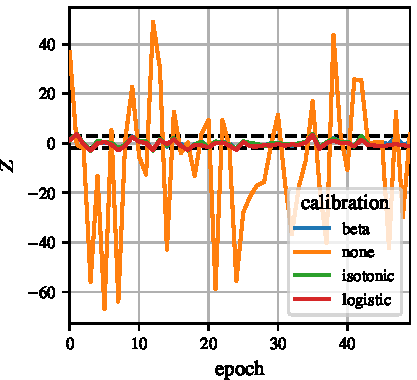
\includegraphics[scale=0.9]{figures/disc_calib.pdf}
       \caption{CIFAR-10}
       \label{fig:calibration cifar}
    \end{subfigure}
    \begin{subfigure}[b]{0.49\textwidth}
       \centering
       % TODO put in new figure here!!
       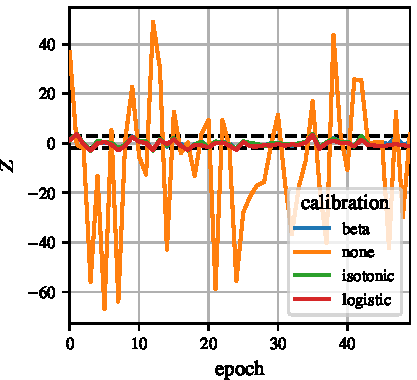
\includegraphics[scale=0.9]{figures/disc_calib.pdf}
       \caption{CelebA}
       \label{fig:calibration CelebA}
    \end{subfigure}
    \caption{{\small
    We show the calibration statistic $Z$ for the discriminator on held out data for the DCGAN\@.
    The results for CIFAR-10 are shown on the right, and CelebA on the left.
    The raw discriminator is clearly miscalibrated being far outside the region expected by chance (dashed black)\@.
    All the calibration methods give roughly equivalent results.
    }}
    \label{fig:calibration}
\end{figure}

